\documentclass[aps, superscriptaddress, notitlepage]{revtex4-1}

\usepackage{amsmath,amsfonts,amssymb,graphicx,hyperref,listings,xcolor,float}
\usepackage[ddmmyyyy, 24hr]{datetime}

% tikz
\usepackage{tikz}
\usetikzlibrary{calc}
\usetikzlibrary{arrows.meta,arrows}

% (pseudo-)algorithms
% https://tex.stackexchange.com/questions/70181
\usepackage{algcompatible,newfloat,etoolbox}
\AtEndEnvironment{algorithm}{\noindent\hrulefill\par\nobreak\vskip-5pt}
\DeclareFloatingEnvironment[fileext=loa, listname=List of Algorithms, name=ALG., placement=tbhp]{algorithm}
% https://tex.stackexchange.com/questions/353132
\algrenewcommand\algorithmicrequire{\textbf{Input:}}
\algrenewcommand\algorithmicensure{\textbf{Output:}}
% https://tex.stackexchange.com/questions/180212
\algrenewcommand{\algorithmiccomment}[2][.6\linewidth]{\leavevmode\hfill\makebox[#1][l]{\triangleright~#2}}
% https://tex.stackexchange.com/questions/184827
\providecommand{\LINECOMMENT}[2][.6\linewidth]{\STATEx\algorithmiccomment[#1]{#2}}
% algorithm macros
\providecommand\RETURN{\STATE\textbf{return}~}
\providecommand\ASSERT{\STATE\textbf{assert}~}

% colours
% seaborn `colorblind' palette
% https://seaborn.pydata.org/tutorial/color_palettes.html
\definecolor{purple}{HTML}{CC78BC}
\definecolor{green}{HTML}{029E73}
\definecolor{blue}{HTML}{0173B2}
\definecolor{lightblue}{HTML}{56B4E9}
\definecolor{yellow}{HTML}{DE8F05}
\definecolor{brown}{HTML}{CA9161}
\definecolor{red}{HTML}{D55E00}
\definecolor{grey}{HTML}{949494}
\definecolor{pink}{HTML}{FBAFE4}
\definecolor{lightyellow}{HTML}{ECE133}

% header/footer
% https://tex.stackexchange.com/questions/117402
\usepackage{fancyhdr} 
\cfoot{\thepage}
\pagestyle{fancy}
% https://tex.stackexchange.com/questions/40172
\renewcommand{\headrulewidth}{0pt}
\fancyhead{}

%%%%% MACROS

\def\scale{0.8}

%%%%% DOCUMENT

\begin{document}

%%%%% TITLE

\title{(Active) vertex model}
\author{Yann-Edwin Keta}
\date{\today, \currenttime}
\maketitle

%%%%% CONTENT

\section{Mesh}

\begin{figure}[H]
\centering
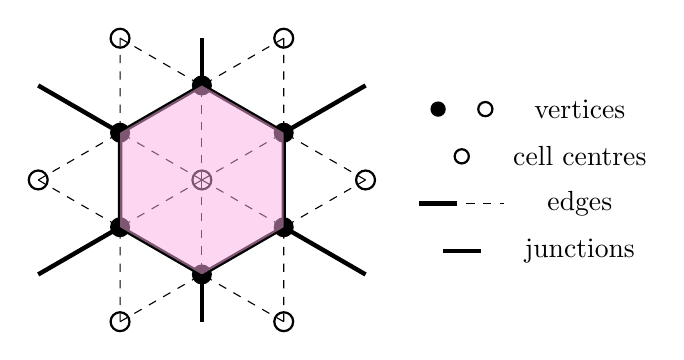
\begin{tikzpicture}[scale=0.75*\scale]
% FIRST CELL
% cell centre
\coordinate (A) at (0, 0);
\draw[thick] (A) circle (0.2);
% cell corners
\coordinate (B) at ($(A) + ({2*cos(30 + 0*60)}, {2*sin(30 + 0*60)})$);
\draw[fill=black] (B) circle (0.2);
\coordinate (C) at ($(A) + ({2*cos(30 + 1*60)}, {2*sin(30 + 1*60)})$);
\draw[fill=black] (C) circle (0.2);
\coordinate (D) at ($(A) + ({2*cos(30 + 2*60)}, {2*sin(30 + 2*60)})$);
\draw[fill=black] (D) circle (0.2);
\coordinate (E) at ($(A) + ({2*cos(30 + 3*60)}, {2*sin(30 + 3*60)})$);
\draw[fill=black] (E) circle (0.2);
\coordinate (F) at ($(A) + ({2*cos(30 + 4*60)}, {2*sin(30 + 4*60)})$);
\draw[fill=black] (F) circle (0.2);
\coordinate (G) at ($(A) + ({2*cos(30 + 5*60)}, {2*sin(30 + 5*60)})$);
\draw[fill=black] (G) circle (0.2);
% junctions
\draw[ultra thick] (B) -- (C) -- (D) -- (E) -- (F) -- (G) -- (B);
% inner edges
\draw[dashed] (A) -- (B);
\draw[dashed] (A) -- (C);
\draw[dashed] (A) -- (D);
\draw[dashed] (A) -- (E);
\draw[dashed] (A) -- (F);
\draw[dashed] (A) -- (G);
% fill
\fill[opacity=0.5, pink] (B) -- (C) -- (D) -- (E) -- (F) -- (G) -- (B);

% SECOND CELL
% cell centre
\coordinate (H) at ($(B) + ({2*cos(30)}, {-2*sin(30)})$);
\draw[thick] (H) circle (0.2);
% cell corners
\coordinate (I) at ($(H) + (0, 2)$);
\coordinate (J) at ($(H) + (0, -2)$);
% juntions
\draw[ultra thick] (B) -- (I);
\draw[ultra thick] (G) -- (J);
% inner edges
\draw[dashed] (H) -- (B);
\draw[dashed] (H) -- (G);

% THIRD CELL
% cell centre
\coordinate (K) at ($(D) + ({-2*cos(30)}, {-2*sin(30)})$);
\draw[thick] (K) circle (0.2);
% cell corners
\coordinate (L) at ($(K) + (0, 2)$);
\coordinate (M) at ($(K) + (0, -2)$);
% juntions
\draw[ultra thick] (D) -- (L);
\draw[ultra thick] (E) -- (M);
% inner edges
\draw[dashed] (K) -- (D);
\draw[dashed] (K) -- (E);

% ADDITIONAL POINTS
\coordinate (N) at ($(C) + (0, 1)$);
\draw[ultra thick] (C) -- (N);
\coordinate (O) at ($(F) + (0, -1)$);
\draw[ultra thick] (F) -- (O);

% ADDITIONAL CELL CENTRES
% cell centre
\coordinate (P) at ($(B) + (0, 2)$);
\draw[thick] (P) circle (0.2);
% inner edges
\draw[dashed] (P) -- (B);
\draw[dashed] (P) -- (C);
% cell centre
\coordinate (Q) at ($(D) + (0, 2)$);
\draw[thick] (Q) circle (0.2);
% inner edges
\draw[dashed] (Q) -- (C);
\draw[dashed] (Q) -- (D);
% cell centre
\coordinate (R) at ($(E) + (0, -2)$);
\draw[thick] (R) circle (0.2);
% inner edges
\draw[dashed] (R) -- (E);
\draw[dashed] (R) -- (F);
% cell centre
\coordinate (S) at ($(G) + (0, -2)$);
\draw[thick] (S) circle (0.2);
% inner edges
\draw[dashed] (S) -- (F);
\draw[dashed] (S) -- (G);

% LEGEND
\draw[fill=black] (5, 1.5) circle (0.15);
\draw[thick] (6, 1.5) circle (0.15);
\draw (8, 1.5) node[]{vertices};
\draw[thick] (5.5, 0.5) circle (0.15);
\draw (8, 0.5) node[]{cell centres};
\draw[ultra thick] (4.6, -0.5) -- ++(0.8, 0);
\draw[dashed] (5.6, -0.5) -- ++(0.8, 0);
\draw (8, -0.5) node[]{edges};
\draw[ultra thick] (5.1, -1.5) -- ++ (0.8, 0);
\draw (8, -1.5) node[]{junctions};

\end{tikzpicture}
\caption{Schematic of a cell (highlighted in pink) in the vertex model.}
\label{fig:schematic}
\end{figure}

A \textit{cell centre} is enclosed by \textit{cell corners} (or \textit{vertices}). These are linked between themselves by \textit{junctions}. We will assume (i) that cells are always convex so that the mesh remains planar, and (ii) that no edge joins two cell centres. The ensemble of the vertices and the edges that link them constitutes the \textit{geometric mesh}. The specification of the cell centres and the junctions between non-cell-centres defines the \textit{physical mesh}.

\section{Cell potential energy}

We introduce for each cell $i$ a reference perimeter $P^0_i$ and a reference area $A^0_i$, and for each of its cell corner $\mu \in \Omega_i$ a force whose effect is to bring the cell's perimeter $P_i$ and area $A_i$ to their reference quantities. A possible force derives from the following potential energy \cite{farhadifar2007influence,fletcher2014vertex,bi2016motilitydriven,sknepnek2023generating}
\begin{equation}
E_{\mathrm{VM}} = \sum_{\text{cells } i} \left[\frac{1}{2} K_i (A_i - A_i^0)^2 + \frac{1}{2} \Gamma_i (P_i - P_i^0)^2\right],
\label{eq:evm}
\end{equation}
where $K_i$ and $\Gamma_i$ are respectively area and perimeter elastic constants. We denote $\boldsymbol{r}_{\mu}$, $\boldsymbol{r}_i$ the position of vertices $\mu, i$. The cell's perimeter can be written
\begin{equation}
P_i = \sum_{\mu \in \Omega_i} |\boldsymbol{r}_{\mu} - \boldsymbol{r}_{\mu - 1}|,
\end{equation}
and the cell's area can be computed with the shoelace formula
\begin{equation}
A_i = \sum_{\mu \in \Omega_i} \frac{1}{2} [(\boldsymbol{r}_{\mu} - \boldsymbol{r}_{i}) \times (\boldsymbol{r}_{\mu - 1} - \boldsymbol{r}_{i})] \cdot \hat{\boldsymbol{e}}_z.
\end{equation}
Note that, by convention of ordering of cell corners, each term in this sum \textit{must be} positive. With these notations, we thus write the force acting on vertex $\mu$
\begin{equation}
\boldsymbol{F}_{\mathrm{VM},\mu} = -\nabla_{\mu} E_{\mathrm{VM}},
\label{eq:fmugrade}
\end{equation}
where $\nabla_{\mu} \equiv \partial/\partial \boldsymbol{r}_{\mu}$. We compute
\begin{equation}
\nabla_{\mu} \left(|\boldsymbol{r}_{\mu} - \boldsymbol{r}_{\mu - 1}|\right) = \frac{\boldsymbol{r}_{\mu} - \boldsymbol{r}_{\mu - 1}}{|\boldsymbol{r}_{\mu} - \boldsymbol{r}_{\mu - 1}|},
\end{equation}
as well as
\begin{equation}
\nabla_{\mu} \left([(\boldsymbol{r}_{\mu} - \boldsymbol{r}_i) \times (\boldsymbol{r}_{\mu - 1} - \boldsymbol{r}_i)] \cdot \hat{\boldsymbol{e}}_z\right) = (\boldsymbol{r}_{\mu - 1} - \boldsymbol{r}_i) \times \hat{\boldsymbol{e}}_z
\end{equation}
to write \eqref{eq:fmugrade} in its full form
\begin{equation}
\begin{aligned}
\boldsymbol{F}_{\mathrm{VM},\mu} &= - \sum_{\text{cells i},~ \mu \in \Omega_i} \bigg[\frac{1}{2} K_i (A_i - A^0_i) \left[(\boldsymbol{r}_{\mu + 1} - \boldsymbol{r}_i) \times \hat{\boldsymbol{e}}_z - (\boldsymbol{r}_{\mu - 1} - \boldsymbol{r}_i) \times \hat{\boldsymbol{e}}_z\right]\\
&\qquad\qquad\qquad\qquad+ \Gamma_i (P_i - P^0_i) \left[\frac{\boldsymbol{r}_{\mu} - \boldsymbol{r}_{\mu - 1}}{|\boldsymbol{r}_{\mu} - \boldsymbol{r}_{\mu - 1}|} + \frac{\boldsymbol{r}_{\mu} - \boldsymbol{r}_{\mu - 1}}{|\boldsymbol{r}_{\mu} - \boldsymbol{r}_{\mu - 1}|}\right]\bigg]\\
&= \sum_{\text{cells i},~ \mu \in \Omega_i} \bigg[\frac{1}{2} K_i (A_i - A^0_i) {\color{blue} \underbrace{(\boldsymbol{r}_{\mu - 1} - \boldsymbol{r}_{\mu + 1}) \times \hat{\boldsymbol{e}}_z}_{\text{towards cell interior}}} + \Gamma_i (P_i - P^0_i) \bigg[{\color{purple} \underbrace{\frac{\boldsymbol{r}_{\mu - 1} - \boldsymbol{r}_{\mu}}{|\boldsymbol{r}_{\mu - 1} - \boldsymbol{r}_{\mu}|}}_{\text{towards neighbour}}} + {\color{purple} \underbrace{\frac{\boldsymbol{r}_{\mu + 1} - \boldsymbol{r}_{\mu}}{|\boldsymbol{r}_{\mu + 1} - \boldsymbol{r}_{\mu}|}}_{\text{towards neighbour}}}\bigg]\bigg],
\end{aligned}
\end{equation}
where underbraced vectors are represented in Fig.~\ref{fig:fmu}. It is noteworthy that, with potential \eqref{eq:evm}, the force acting on each cell centre is zero
\begin{equation}
\boldsymbol{F}_{\mathrm{VM}, i} = - \nabla_i E_{\mathrm{VM}} = - \frac{1}{2} K_i (A_i - A^0_i) \sum_{\mu \in \Omega_i} (\boldsymbol{r}_{\mu} - \boldsymbol{r}_{\mu - 1}) \times \hat{\boldsymbol{e}}_z = 0.
\end{equation}

\begin{figure}[!t]
\centering
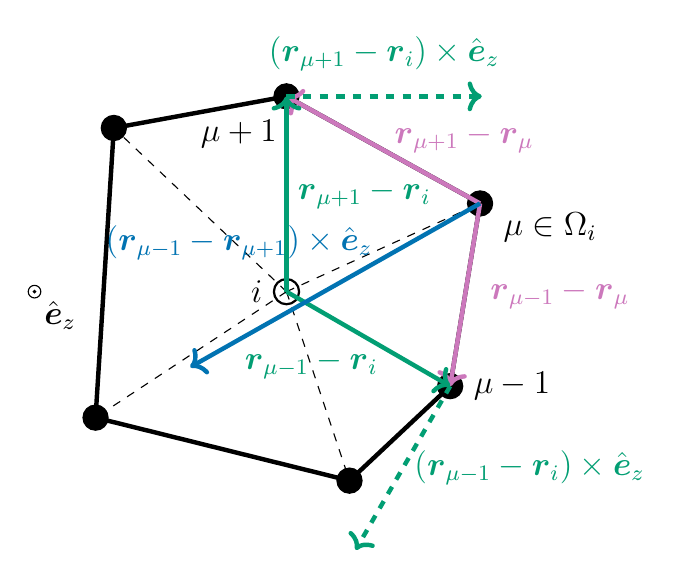
\begin{tikzpicture}[scale=\scale]
% FIRST CELL
% cell centre
\coordinate (A) at (0, 0);
\draw[thick] (A) circle (0.2) node[left,xshift=-5pt]{\large $i$};
% cell corners
\coordinate (B) at ($(A) + ({4*cos(30 + 0.2*60) + 0.1}, {3*sin(30 + 0*60) - 0.1})$);
\draw[fill=black] (B) circle (0.2) node[below right,xshift=5pt]{\large $\mu \in \Omega_i$};
\coordinate (C) at ($(A) + ({2.9*cos(30 + 1*60)}, {3.1*sin(30 + 1*60)})$);
\draw[fill=black] (C) circle (0.2) node[below left,yshift=-5pt]{\large $\mu + 1$};
\coordinate (D) at ($(A) + ({3*cos(30 + 2.1*60)}, {3*sin(30 + 1.5*60)})$);
\draw[fill=black] (D) circle (0.2);
\coordinate (E) at ($(A) + ({3.5*cos(30 + 3*60)}, {4*sin(30 + 3*60)})$);
\draw[fill=black] (E) circle (0.2);
\coordinate (F) at ($(A) + ({1 + 3*cos(30 + 4*60)}, {3*sin(30 + 4*60)})$);
\draw[fill=black] (F) circle (0.2);
\coordinate (G) at ($(A) + ({3*cos(30 + 5*60)}, {3*sin(30 + 5*60)})$);
\draw[fill=black] (G) circle (0.2) node[right,xshift=5pt]{\large $\mu - 1$};
% junctions
\draw[ultra thick] (B) -- (C) -- (D) -- (E) -- (F) -- (G) -- (B);
% inner edges
\draw[dashed] (A) -- (B);
\draw[dashed] (A) -- (C);
\draw[dashed] (A) -- (D);
\draw[dashed] (A) -- (E);
\draw[dashed] (A) -- (F);
\draw[dashed] (A) -- (G);

\draw (-4, 0) circle (0.1) node[below right]{\large $\hat{\boldsymbol{e}}_z$};
\draw[fill=black] (-4, 0) circle (0.02);

% perimeter term
\draw[purple, ultra thick, ->] (B) -- (C) node[midway, above right, xshift=0pt, yshift=-5pt]{\large $\boldsymbol{r}_{\mu + 1} - \boldsymbol{r}_{\mu}$};
\draw[purple, ultra thick, ->] (B) -- (G) node[midway, right, xshift=5pt]{\large $\boldsymbol{r}_{\mu - 1} - \boldsymbol{r}_{\mu}$};

% area term
\draw[green, ultra thick, ->] (A) -- (C) node[midway, right]{\large $\boldsymbol{r}_{\mu + 1} - \boldsymbol{r}_i$};
\draw[green, ultra thick, ->] (A) -- (G) node[midway, below left, xshift=7.5pt]{\large $\boldsymbol{r}_{\mu - 1} - \boldsymbol{r}_i$};
% https://tex.stackexchange.com/a/63569
\draw[green, ultra thick, dashed, ->] let \p{A}=(A), \p{C}=(C) in (C) -- ++({\y{C} - \y{A}}, {-(\x{C} - \x{A})}) node[midway, above, yshift=5pt]{\large $(\boldsymbol{r}_{\mu + 1} - \boldsymbol{r}_i) \times \hat{\boldsymbol{e}}_z$};
\draw[green, ultra thick, dashed, ->] let \p{A}=(A), \p{G}=(G) in (G) -- ++({\y{G} - \y{A}}, {-(\x{G} - \x{A})}) node[midway, right, yshift=0pt]{\large $(\boldsymbol{r}_{\mu - 1} - \boldsymbol{r}_i) \times \hat{\boldsymbol{e}}_z$};
\draw[blue, ultra thick, ->] let \p{C}=(C), \p{G}=(G) in (B) -- ++({-(\y{C} - \y{G})}, {(\x{C} - \x{G})}) node[midway, above left, xshift=17.5pt, yshift=5pt]{\large $(\boldsymbol{r}_{\mu - 1} - \boldsymbol{r}_{\mu + 1}) \times \hat{\boldsymbol{e}}_z$};

\end{tikzpicture}
\caption{Vertex representation of a single cell. By convention, cell centres are denoted by latin indices, and cell corners are denotes by greek indices. We denote $\Omega_i$ the ensemble of cell corners $\mu$ of the cell whose centre is $i$. By convention, $\mu + 1$ (respectively $\mu - 1$) denotes the next cell corner of $i$ after $\mu$ in anticlockwise (respectively clockwise) order.}
\label{fig:fmu}
\end{figure}

\section{Half-edge procedure}

The edges of the mesh (Fig.~\ref{fig:schematic}) divide the entire system in adjacent and non-overlapping \textit{triangles} (or \textit{faces}). We endow all of these triangles with three arrows. These are oriented such that, for an arbitrary vertex (\textit{e.g.}, $\mu$ in Fig.~\ref{fig:he}) and an arbitrary triangle (\textit{e.g.}, $(\mu, \nu, i)$), the cross product of the half-edges pointing toward this vertex in this triangle (\textit{i.e.}, $i \to \mu$) on the one hand and the half-edge pointing out of this vertex in this triangle (\textit{i.e.}, $\mu \to \nu$) on the other hand, has a positive scalar product with $\hat{\boldsymbol{e}}_z$. We introduce three relations between half-edges, which we exemplify in Fig.~\ref{fig:he} using an arbitrary {\color{yellow} reference half-egde $\mu \to \nu$}.
\begin{enumerate}
    \item The {\color{purple} \textit{next} half-edge} departs from the vertex pointed at by the reference half-edge (\textit{i.e.}, $\nu$ here) inside the same triangle. ``Next'' is an order-3 bijection, meaning that the next half-edge of the next half-edge of any half-edge is this same half-edge.
    \item The {\color{green} \textit{previous} half-edge} points towards the vertex from which departs the reference half-edge (\textit{i.e.}, $\mu$ here) inside the same triangle. ``Previous'' is also an order-3 bijection.
    \item The {\color{blue} \textit{pair} half-edge} has inverse depart and arrival vertices with respect to the reference half-edge (\textit{i.e.}, $\nu$ and $\mu$ here) in the adjacent triangle sharing the same edge the reference half-edge belongs to. ``Pair'' is an order-2 bijecton, meaning that the pair half-edge of any pair half-edge is this same half-edge.
\end{enumerate}
These relations between the half-edges enable us to identify all neighbours of any vertex (Alg.~\ref{alg:neighbours}), given that each vertex contains the information of (at least) one half-edge leaving the vertex. We propose in Alg.~\ref{alg:check} a way to check the consistency of the half-edge construction in the mesh.

\begin{figure}[!t]
\centering
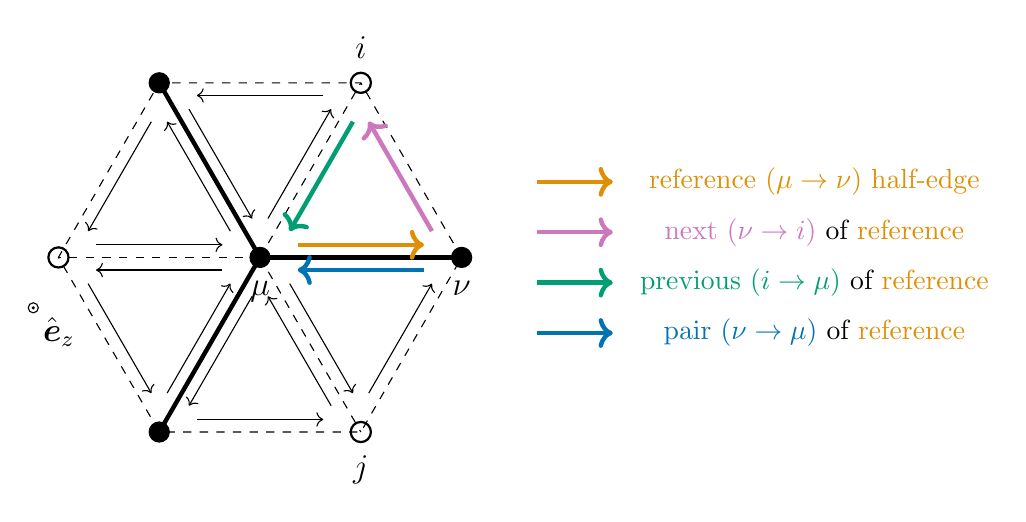
\begin{tikzpicture}[scale=0.8*\scale]
% vertices

\coordinate (A) at (0, 0);
\draw[fill=black] (A) circle (0.2) node[below, yshift=-5pt]{\large $\mu$};

\coordinate (B) at ($(A) + ({4*cos(0*60)}, {4*sin(0*60)})$);
\draw[fill=black] (B) circle (0.2) node[below, yshift=-5pt]{\large $\nu$};
\coordinate (C) at ($(A) + ({4*cos(1*60)}, {4*sin(1*60)})$);
\draw[thick] (C) circle (0.2) node[above, yshift=5pt]{\large $i$};
\coordinate (D) at ($(A) + ({4*cos(2*60)}, {4*sin(2*60)})$);
\draw[fill=black] (D) circle (0.2);
\coordinate (E) at ($(A) + ({4*cos(3*60)}, {4*sin(3*60)})$);
\draw[thick] (E) circle (0.2);
\coordinate (F) at ($(A) + ({4*cos(4*60)}, {4*sin(4*60)})$);
\draw[fill=black] (F) circle (0.2);
\coordinate (G) at ($(A) + ({4*cos(5*60)}, {4*sin(5*60)})$);
\draw[thick] (G) circle (0.2) node[below, yshift=-5pt]{\large $j$};

% edges

\draw[dashed] (B) -- (C) -- (D) -- (E) -- (F) -- (G) -- (B);

\draw[ultra thick] (A) -- (B);
\draw[dashed] (A) -- (C);
\draw[ultra thick] (A) -- (D);
\draw[dashed] (A) -- (E);
\draw[ultra thick] (A) -- (F);
\draw[dashed] (A) -- (G);

% intermediate points
\path (A) +({30 + 0*60}:0.5) coordinate (A0);
\path (A) +({30 + 1*60}:0.5) coordinate (A1);
\path (A) +({30 + 2*60}:0.5) coordinate (A2);
\path (A) +({30 + 3*60}:0.5) coordinate (A3);
\path (A) +({30 + 4*60}:0.5) coordinate (A4);
\path (A) +({30 + 5*60}:0.5) coordinate (A5);
\path (B) +({180 + 0*60 + 30}:0.5) coordinate (B0);
\path (B) +({180 + 0*60 - 30}:0.5) coordinate (B1);
\path (C) +({180 + 1*60 + 30}:0.5) coordinate (C0);
\path (C) +({180 + 1*60 - 30}:0.5) coordinate (C1);
\path (D) +({180 + 2*60 + 30}:0.5) coordinate (D0);
\path (D) +({180 + 2*60 - 30}:0.5) coordinate (D1);
\path (E) +({180 + 3*60 + 30}:0.5) coordinate (E0);
\path (E) +({180 + 3*60 - 30}:0.5) coordinate (E1);
\path (F) +({180 + 4*60 + 30}:0.5) coordinate (F0);
\path (F) +({180 + 4*60 - 30}:0.5) coordinate (F1);
\path (G) +({180 + 5*60 + 30}:0.5) coordinate (G0);
\path (G) +({180 + 5*60 - 30}:0.5) coordinate (G1);

% first triangle
\draw[ultra thick, yellow, ->] ($(A0)!0.1!(B1)$) -- ($(A0)!0.9!(B1)$);
\draw[ultra thick, purple, ->] ($(B1)!0.1!(C0)$) -- ($(B1)!0.9!(C0)$);
\draw[ultra thick, green, ->] ($(C0)!0.1!(A0)$) -- ($(C0)!0.9!(A0)$);
% second triangle
\draw[->] ($(A1)!0.1!(C1)$) -- ($(A1)!0.9!(C1)$);
\draw[->] ($(C1)!0.1!(D0)$) -- ($(C1)!0.9!(D0)$);
\draw[->] ($(D0)!0.1!(A1)$) -- ($(D0)!0.9!(A1)$);
% third triangle
\draw[->] ($(A2)!0.1!(D1)$) -- ($(A2)!0.9!(D1)$);
\draw[->] ($(D1)!0.1!(E0)$) -- ($(D1)!0.9!(E0)$);
\draw[->] ($(E0)!0.1!(A2)$) -- ($(E0)!0.9!(A2)$);
% fourth triangle
\draw[->] ($(A3)!0.1!(E1)$) -- ($(A3)!0.9!(E1)$);
\draw[->] ($(E1)!0.1!(F0)$) -- ($(E1)!0.9!(F0)$);
\draw[->] ($(F0)!0.1!(A3)$) -- ($(F0)!0.9!(A3)$);
% fifth triangle
\draw[->] ($(A4)!0.1!(F1)$) -- ($(A4)!0.9!(F1)$);
\draw[->] ($(F1)!0.1!(G0)$) -- ($(F1)!0.9!(G0)$);
\draw[->] ($(G0)!0.1!(A4)$) -- ($(G0)!0.9!(A4)$);
% sixth triangle
\draw[->] ($(A5)!0.1!(G1)$) -- ($(A5)!0.9!(G1)$);
\draw[->] ($(G1)!0.1!(B0)$) -- ($(G1)!0.9!(B0)$);
\draw[ultra thick, blue, ->] ($(B0)!0.1!(A5)$) -- ($(B0)!0.9!(A5)$);

% LEGEND
\draw[ultra thick, yellow, ->] (5.5, 1.5) -- +(1.5, 0);
\draw[ultra thick, purple, ->] (5.5, 0.5) -- +(1.5, 0);
\draw[ultra thick, green, ->] (5.5, -0.5) -- +(1.5, 0);
\draw[ultra thick, blue, ->] (5.5, -1.5) -- +(1.5, 0);
\draw (11, 1.5) node[]{\color{yellow} reference ($\mu \to \nu$) half-edge};
\draw (11, 0.5) node[]{{\color{purple} next ($\nu \to i$)} of {\color{yellow} reference}};
\draw (11, -0.5) node[]{{\color{green} previous ($i \to \mu$)} of {\color{yellow} reference}};
\draw (11, -1.5) node[]{{\color{blue} pair ($\nu \to \mu$)} of {\color{yellow} reference}};

\draw (-4.5, -1) circle (0.1) node[below right]{\large $\hat{\boldsymbol{e}}_z$};
\draw[fill=black] (-4.5, -1) circle (0.02);

\end{tikzpicture}
\caption{Half-edge representation in 6 adjacent triangles, highlighting an arbitrary reference half-edge and its associated half-edges.}
\label{fig:he}
\end{figure}

\section{T1 transition}

T1 transitions correspond to changes in the mesh topology (Fig.~\ref{fig:t1}).

\begin{figure}[H]
\centering
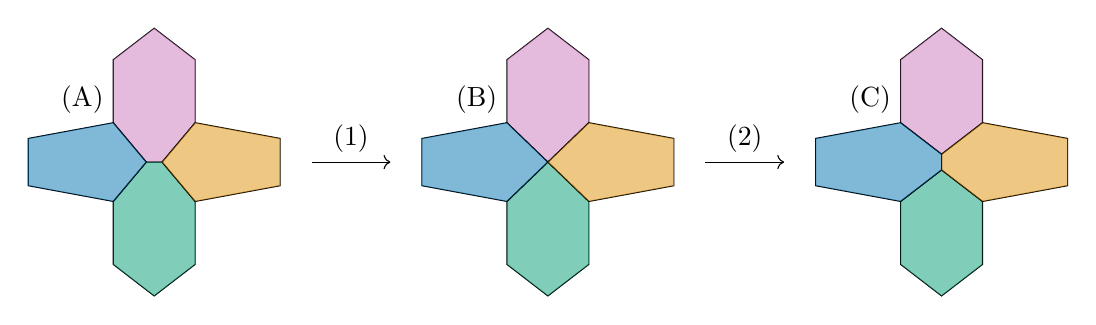
\begin{tikzpicture}[scale=0.25*\scale]
% before T1

\coordinate (A'') at (0, 2);
\coordinate (B'') at ($(A'') + ({4*cos(0*60 - 90)}, {4*sin(0*60 - 90)})$);
\coordinate (C'') at ($(A'') + ({3*cos(1*60 - 90)}, {4*sin(1*60 - 90)})$);
\coordinate (D'') at ($(A'') + ({3*cos(2*60 - 90)}, {4*sin(2*60 - 90)})$);
\coordinate (E'') at ($(A'') + ({4*cos(3*60 - 90)}, {4*sin(3*60 - 90)})$);
\coordinate (F'') at ($(A'') + ({3*cos(4*60 - 90)}, {4*sin(4*60 - 90)})$);
\coordinate (G'') at ($(A'') + ({3*cos(5*60 - 90)}, {4*sin(5*60 - 90)})$);

\coordinate (H'') at (0, -7);
\coordinate (I'') at ($(H'') + ({4*cos(0*60 - 90)}, {4*sin(0*60 - 90)})$);
\coordinate (J'') at ($(H'') + ({3*cos(1*60 - 90)}, {4*sin(1*60 - 90)})$);
\coordinate (K'') at ($(H'') + ({3*cos(2*60 - 90)}, {4*sin(2*60 - 90)})$);
\coordinate (L'') at ($(H'') + ({4*cos(3*60 - 90)}, {4*sin(3*60 - 90)})$);
\coordinate (M'') at ($(H'') + ({3*cos(4*60 - 90)}, {4*sin(4*60 - 90)})$);
\coordinate (N'') at ($(H'') + ({3*cos(5*60 - 90)}, {4*sin(5*60 - 90)})$);

\coordinate (Z') at (-0.5, -2.5);
\coordinate (Z'') at (0.5, -2.5);

\coordinate (P'') at ($(B'') + (-8, 1)$);
\coordinate (Q'') at ($(L'') + (-8, -1)$);

\coordinate (R'') at ($(B'') + (8, 1)$);
\coordinate (S'') at ($(L'') + (8, -1)$);

\draw (Z') -- (Z'') -- (C'') -- (D'') -- (E'') -- (F'') -- (G'') -- cycle;
\fill[opacity=0.5, purple] (Z') -- (Z'') -- (C'') -- (D'') -- (E'') -- (F'') -- (G'') -- cycle;

\draw (I'') -- (J'') -- (K'') -- (Z'') -- (Z') -- (M'') -- (N'') -- cycle;
\fill[opacity=0.5, green] (I'') -- (J'') -- (K'') -- (Z'') -- (Z') -- (M'') -- (N'') -- cycle;

\draw (Z') -- (G'') -- (P'') -- (Q'') -- (M'') -- cycle;
\fill[opacity=0.5, blue] (Z') -- (G'') -- (P'') -- (Q'') -- (M'') -- cycle;

\draw (K'') -- (S'') -- (R'') -- (C'') -- (Z'') -- cycle;
\fill[opacity=0.5, yellow] (K'') -- (S'') -- (R'') -- (C'') -- (Z'') -- cycle;

% 4-vertex

\coordinate (A') at (25, 2);
\coordinate (B') at ($(A') + ({4*cos(0*60 - 90)}, {4*sin(0*60 - 90)})$);
\coordinate (C') at ($(A') + ({3*cos(1*60 - 90)}, {4*sin(1*60 - 90)})$);
\coordinate (D') at ($(A') + ({3*cos(2*60 - 90)}, {4*sin(2*60 - 90)})$);
\coordinate (E') at ($(A') + ({4*cos(3*60 - 90)}, {4*sin(3*60 - 90)})$);
\coordinate (F') at ($(A') + ({3*cos(4*60 - 90)}, {4*sin(4*60 - 90)})$);
\coordinate (G') at ($(A') + ({3*cos(5*60 - 90)}, {4*sin(5*60 - 90)})$);

\coordinate (H') at (25, -7);
\coordinate (I') at ($(H') + ({4*cos(0*60 - 90)}, {4*sin(0*60 - 90)})$);
\coordinate (J') at ($(H') + ({3*cos(1*60 - 90)}, {4*sin(1*60 - 90)})$);
\coordinate (K') at ($(H') + ({3*cos(2*60 - 90)}, {4*sin(2*60 - 90)})$);
\coordinate (L') at ($(H') + ({4*cos(3*60 - 90)}, {4*sin(3*60 - 90)})$);
\coordinate (M') at ($(H') + ({3*cos(4*60 - 90)}, {4*sin(4*60 - 90)})$);
\coordinate (N') at ($(H') + ({3*cos(5*60 - 90)}, {4*sin(5*60 - 90)})$);

\coordinate (Z) at ($(B')!0.5!(L')$);

\coordinate (P') at ($(B') + (-8, 1)$);
\coordinate (Q') at ($(L') + (-8, -1)$);

\coordinate (R') at ($(B') + (8, 1)$);
\coordinate (S') at ($(L') + (8, -1)$);

\draw (Z) -- (C') -- (D') -- (E') -- (F') -- (G') -- cycle;
\fill[opacity=0.5, purple] (Z) -- (C') -- (D') -- (E') -- (F') -- (G') -- cycle;

\draw (I') -- (J') -- (K') -- (Z) -- (M') -- (N') -- cycle;
\fill[opacity=0.5, green] (I') -- (J') -- (K') -- (Z) -- (M') -- (N') -- cycle;

\draw (Z) -- (G') -- (P') -- (Q') -- (M') -- cycle;
\fill[opacity=0.5, blue] (Z) -- (G') -- (P') -- (Q') -- (M') -- cycle;

\draw (K') -- (S') -- (R') -- (C') -- (Z) -- cycle;
\fill[opacity=0.5, yellow] (K') -- (S') -- (R') -- (C') -- (Z) -- cycle;

% after T1

\coordinate (A) at (50, 2);
\coordinate (B) at ($(A) + ({4*cos(0*60 - 90)}, {4*sin(0*60 - 90)})$);
\coordinate (C) at ($(A) + ({3*cos(1*60 - 90)}, {4*sin(1*60 - 90)})$);
\coordinate (D) at ($(A) + ({3*cos(2*60 - 90)}, {4*sin(2*60 - 90)})$);
\coordinate (E) at ($(A) + ({4*cos(3*60 - 90)}, {4*sin(3*60 - 90)})$);
\coordinate (F) at ($(A) + ({3*cos(4*60 - 90)}, {4*sin(4*60 - 90)})$);
\coordinate (G) at ($(A) + ({3*cos(5*60 - 90)}, {4*sin(5*60 - 90)})$);
\draw (B) -- (C) -- (D) -- (E) -- (F) -- (G) -- cycle;
\fill[opacity=0.5, purple] (B) -- (C) -- (D) -- (E) -- (F) -- (G) -- cycle;

\coordinate (H) at (50, -7);
\coordinate (I) at ($(H) + ({4*cos(0*60 - 90)}, {4*sin(0*60 - 90)})$);
\coordinate (J) at ($(H) + ({3*cos(1*60 - 90)}, {4*sin(1*60 - 90)})$);
\coordinate (K) at ($(H) + ({3*cos(2*60 - 90)}, {4*sin(2*60 - 90)})$);
\coordinate (L) at ($(H) + ({4*cos(3*60 - 90)}, {4*sin(3*60 - 90)})$);
\coordinate (M) at ($(H) + ({3*cos(4*60 - 90)}, {4*sin(4*60 - 90)})$);
\coordinate (N) at ($(H) + ({3*cos(5*60 - 90)}, {4*sin(5*60 - 90)})$);
\draw (I) -- (J) -- (K) -- (L) -- (M) -- (N) -- cycle;
\fill[opacity=0.5, green] (I) -- (J) -- (K) -- (L) -- (M) -- (N) -- cycle;

\coordinate (P) at ($(B) + (-8, 1)$);
\coordinate (Q) at ($(L) + (-8, -1)$);
\draw (L) -- (B) -- (G) -- (P) -- (Q) -- (M) -- cycle;
\fill[opacity=0.5, blue] (L) -- (B) -- (G) -- (P) -- (Q) -- (M) -- cycle;

\coordinate (R) at ($(B) + (8, 1)$);
\coordinate (S) at ($(L) + (8, -1)$);
\draw (K) -- (S) -- (R) -- (C) -- (B) -- (L) -- cycle;
\fill[opacity=0.5, yellow] (K) -- (S) -- (R) -- (C) -- (B) -- (L) -- cycle;

% arrows

\draw (G'') node[above left]{(A)};
\draw (G') node[above left]{(B)};
\draw (G) node[above left]{(C)};
\draw[->] (10, -2.5) -- ++(5, 0) node[midway, above]{(1)};
\draw[->] (35, -2.5) -- ++(5, 0) node[midway, above]{(2)};

\end{tikzpicture}
\caption{}
\label{fig:t1}
\end{figure}

\begin{figure}[H]
\centering
\begin{tikzpicture}[scale=0.75*\scale]
\input{src/merge}
\end{tikzpicture}
\caption{}
\label{fig:merge}
\end{figure}

\begin{figure}[H]
\centering
\begin{tikzpicture}[scale=0.75*\scale]
\input{src/create}
\end{tikzpicture}
\caption{}
\label{fig:create}
\end{figure}

\bibliography{ref}

\newpage
\appendix

\section{Algorithms}

\begin{algorithm}[H]
\caption{Find all neighbours of an arbitrary vertex and all half-edges from this vertex to its neighbours. All vertices (cell centre or not) are denoted with latin indices.}
\label{alg:neighbours}
\begin{algorithmic}[1]
\REQUIRE Arbitrary half-edge $\boldsymbol{h}$ departing from a given vertex $v$.
\ENSURE Ensemble $\mathcal{D}$ of neighbours of vertex $v$, ensemble $\mathcal{H}$ of half-edges from vertex $v$ to its neighbours.
\STATE{Set $d^0 = $ destination vertex of $\boldsymbol{h}$.} \COMMENT[0.7\textwidth]{Save first neighbour.}
\STATE{Set $d = \textsc{null}$.} \COMMENT[0.7\textwidth]{Setting to \textsc{null} to enter while loop \ref{ins:while_neigh}.}
\WHILE{$d \neq d^0$}
\label{ins:while_neigh}
    \STATE{Set $\boldsymbol{h} =$ pair half-edge of previous half-edge of $\boldsymbol{h}$.}
    \STATE{Set $d =$ destination vectex of $\boldsymbol{h}$.}
    \STATE{Add $d$ to $\mathcal{D}$, add $\boldsymbol{h}$ to $\mathcal{H}$.} \COMMENT[0.7\textwidth]{By convention of the half-edge construction, these are added in anticlockwise order.}
\ENDWHILE
\RETURN $\mathcal{D},~\mathcal{H}$
\end{algorithmic}
\end{algorithm}

\begin{algorithm}[H]
\caption{Check half-edge construction.}
\label{alg:check}
\begin{algorithmic}[1]
\REQUIRE Ensemble $\mathcal{V}$ of all vertices, ensemble $\mathcal{H}$ of all half-edges.
\STATE{Make copies $\mathcal{V}^{\prime}$ and $\mathcal{H}^{\prime}$ of $\mathcal{V}$ and $\mathcal{H}$.}
\FOR{$\boldsymbol{h} \in \mathcal{H}$}
    \IF{$\boldsymbol{h} \notin \mathcal{H}^{\prime}$} \COMMENT{Half-edge $\boldsymbol{h}$ has already been checked.}
        \STATE{\textbf{continue}}
    \ENDIF
    \STATE{Set $\mathcal{T} = \{\boldsymbol{h},~\text{next of }\boldsymbol{h},~\text{previous of }\boldsymbol{h}\}$.} \COMMENT{Triangle to which $\boldsymbol{h}$ belongs.}
    \FOR{$\boldsymbol{h}^{\prime} \in \mathcal{T}$} \COMMENT{Loop over the half-edges in the triangle.}
        \STATE{Set $o$ and $d$ as the origin and destination vertices of $\boldsymbol{h}^{\prime}$.}
        \IF{$o \in \mathcal{V}^{\prime}$} \COMMENT{Origin vertex $o$ has not been checked.}
            \ASSERT $o$ knows one half-edge which \textit{does} leave from $o$
            \STATE{Remove $o$ from $\mathcal{V}^{\prime}$.}
        \ENDIF
        \ASSERT $[\boldsymbol{h}^{\prime} \times (\boldsymbol{h}^{\prime} + 1)] \cdot \hat{\boldsymbol{e}}_z > 0$ \COMMENT{Check orientation, $\boldsymbol{h}^{\prime} + 1$ is meant as next element in order in $\mathcal{T}$.}
        \ASSERT pair half-edge of $\boldsymbol{h}^{\prime}$ has opposite origin and destination vertices \COMMENT[0.35\textwidth]{Check half-edge.}
        \ASSERT $\boldsymbol{h}^{\prime}$ is the pair of half-edge of its pair half-edge
        \ASSERT $\boldsymbol{h}^{\prime}$ is previous half-edge of $\boldsymbol{h}^{\prime} + 1$. \COMMENT[0.35\textwidth]{Check next half-edge.}
        \ASSERT destination vertex of $\boldsymbol{h}^{\prime}$ is the origin vertex of $\boldsymbol{h}^{\prime} + 1$
        \ASSERT $\boldsymbol{h}^{\prime}$ is next half-edge of $\boldsymbol{h}^{\prime} - 1$. \COMMENT[0.35\textwidth]{Check previous half-edge.}
        \ASSERT origin vertex of $\boldsymbol{h}^{\prime}$ is the destination vertex of $\boldsymbol{h}^{\prime} - 1$
        \STATE{Remove $\boldsymbol{h}^{\prime}$ from $\mathcal{H}^{\prime}$.}
    \ENDFOR
\ENDFOR
\ASSERT $\mathcal{V}^{\prime} = \emptyset$ and $\mathcal{H}^{\prime} = \emptyset$
\end{algorithmic}
\end{algorithm}

\end{document}

